\documentclass{article}
\usepackage{amsfonts}
\usepackage{amsmath}
\usepackage{amssymb}
\usepackage{hyperref}
\usepackage{mathrsfs}
\usepackage{tikz}

\parindent=0pt

\usetikzlibrary{positioning}

\def\upint{\mathchoice%
    {\mkern13mu\overline{\vphantom{\intop}\mkern7mu}\mkern-20mu}%
    {\mkern7mu\overline{\vphantom{\intop}\mkern7mu}\mkern-14mu}%
    {\mkern7mu\overline{\vphantom{\intop}\mkern7mu}\mkern-14mu}%
    {\mkern7mu\overline{\vphantom{\intop}\mkern7mu}\mkern-14mu}%
  \int}
\def\lowint{\mkern3mu\underline{\vphantom{\intop}\mkern7mu}\mkern-10mu\int}

\begin{document}

\textbf{\Large Chapter 2: Modules} \\\\



\emph{Author: Meng-Gen Tsai} \\
\emph{Email: plover@gmail.com} \\\\



% https://metaphor.ethz.ch/x/2018/hs/401-3132-00L/ex/sol_4.pdf



\textbf{Exercise 2.1.}
\emph{Show that
$(\mathbb{Z}/m\mathbb{Z}) \otimes_{\mathbb{Z}} (\mathbb{Z}/n\mathbb{Z}) = 0$
if $m$, $n$ are coprime.} \\

It suffices to show that
$$(\mathbb{Z}/m\mathbb{Z}) \otimes_{\mathbb{Z}} (\mathbb{Z}/n\mathbb{Z})
\cong \mathbb{Z}/d\mathbb{Z}$$
where $d$ is the greatest common divisor of $m$ and $n$. \\

\emph{Outlines.}
\begin{enumerate}
\item[(1)]
Define $\widetilde{\varphi}$ by
\begin{center}
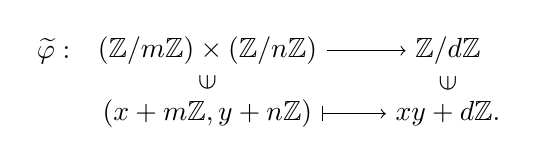
\begin{tikzpicture}[node distance=1mm]
  \node (functionName) at (0, 0) {$\widetilde{\varphi}:$};
  \node[right = of functionName] (domain)
    {$(\mathbb{Z}/m\mathbb{Z}) \times (\mathbb{Z}/n\mathbb{Z})$};
  \node[below = 2mm of domain] (element) {$(x + m\mathbb{Z}, y + n\mathbb{Z})$};
  \path (element)--(domain)node[midway,sloped] {$\in$};
  \node[right = 1cm of domain] (codomain) {$\mathbb{Z}/d\mathbb{Z}$};
  \node at (element-|codomain) (image) {$xy + d\mathbb{Z}.$};
  \path (image)--(codomain)node[midway,sloped] {$\in$};
  \draw[->] (domain) -- (codomain);
  \draw[|->] (element) -- (image);
\end{tikzpicture}
\end{center}
$\widetilde{\varphi}$ is well-defined and $\mathbb{Z}$-bilinear.
\item[(2)]
By the universal property,
$\widetilde{\varphi}$ factors through a $\mathbb{Z}$-bilinear map
$$\varphi: (\mathbb{Z}/m\mathbb{Z}) \otimes_{\mathbb{Z}} (\mathbb{Z}/n\mathbb{Z})
\to \mathbb{Z}/d\mathbb{Z}$$
(such that $\varphi(x \otimes y) = \widetilde{\varphi}(x, y)$).
\item[(3)]
To show that $\varphi$ is isomorphic, might find the inverse map
$\psi: \mathbb{Z}/d\mathbb{Z}
\to
(\mathbb{Z}/m\mathbb{Z}) \otimes_{\mathbb{Z}} (\mathbb{Z}/n\mathbb{Z})$
of $\varphi$.
Define $\psi$ by
\begin{center}
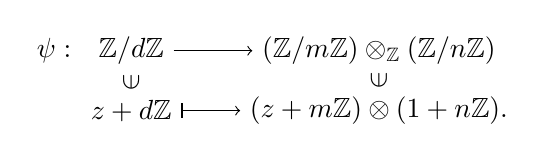
\begin{tikzpicture}[node distance=1mm]
  \node (functionName) at (0, 0) {$\psi:$};
  \node[right = of functionName] (domain) {$\mathbb{Z}/d\mathbb{Z}$};
  \node[below = 2mm of domain] (element) {$z + d\mathbb{Z}$};
  \path (element)--(domain)node[midway,sloped] {$\in$};
  \node[right = 1cm of domain] (codomain)
    {$(\mathbb{Z}/m\mathbb{Z}) \otimes_{\mathbb{Z}} (\mathbb{Z}/n\mathbb{Z})$};
  \node at (element-|codomain) (image) {$(z + m\mathbb{Z}) \otimes (1 + n\mathbb{Z}).$};
  \path (image)--(codomain)node[midway,sloped] {$\in$};
  \draw[->] (domain) -- (codomain);
  \draw[|->] (element) -- (image);
\end{tikzpicture}
\end{center}
$\psi$ is well-defined and $\mathbb{Z}$-linear.
\item[(4)]
$\psi \circ \varphi = \text{id}$.
\item[(5)]
$\varphi \circ \psi = \text{id}$. \\
\end{enumerate}

\emph{Proof of (1).}
\begin{enumerate}
\item[(a)]
\emph{$\widetilde{\varphi}$ is well-defined.}
Say $x' = x + am$ for some $a \in \mathbb{Z}$
and $y' = y + bn$ for some $b \in \mathbb{Z}$.
Then $x'y' - xy = yam + xbn + abmn \in \mathbb{Z}/d\mathbb{Z}$.
That is, $\widetilde{\varphi}$
is independent of coset representative.
\item[(b)]
\emph{$\widetilde{\varphi}$ is $\mathbb{Z}$-bilinear.}
\begin{enumerate}
\item[(i)]
\emph{For any $\lambda \in \mathbb{Z}$,
$\widetilde{\varphi}(\lambda x, y)
= \widetilde{\varphi}(x, \lambda y)
= \lambda \widetilde{\varphi}(x, y)$.}
In fact,
\begin{align*}
  \widetilde{\varphi}(\lambda(x+m\mathbb{Z}), y+n\mathbb{Z})
  &= \widetilde{\varphi}(\lambda x+m\mathbb{Z}, y+n\mathbb{Z})
  = \lambda x y + d\mathbb{Z}, \\
  \widetilde{\varphi}(x+m\mathbb{Z}, \lambda(y+n\mathbb{Z}))
  &= \widetilde{\varphi}(x+m\mathbb{Z}, \lambda y+n\mathbb{Z})
  = \lambda x y + d\mathbb{Z}, \\
  \widetilde{\varphi}(x_1+m\mathbb{Z}, y+n\mathbb{Z})
  &= \lambda (x y + d\mathbb{Z})
  = \lambda x y + d\mathbb{Z}.
\end{align*}
\item[(ii)]
\emph{$\widetilde{\varphi}(x_1 + x_2, y)
= \widetilde{\varphi}(x_1, y) + \widetilde{\varphi}(x_2, y)$.}
In fact,
\begin{align*}
  \widetilde{\varphi}((x_1+x_2)+m\mathbb{Z}, y+n\mathbb{Z})
  &= (x_1 + x_2) y + d\mathbb{Z}, \\
  \widetilde{\varphi}(x_1+m\mathbb{Z}, y+n\mathbb{Z})
  + \widetilde{\varphi}(x_2+m\mathbb{Z}, y+n\mathbb{Z})
  &= (x_1 y + d\mathbb{Z}) + (x_2 y + d\mathbb{Z}) \\
  &= (x_1 + x_2) y + d\mathbb{Z}.
\end{align*}
\item[(iii)]
\emph{$\widetilde{\varphi}(x, y_1 + y_2)
= \widetilde{\varphi}(x, y_1) + \widetilde{\varphi}(x, y_2)$.}
Similar to (ii).
\end{enumerate}
\end{enumerate}
$\Box$ \\

\emph{Proof of (3).}
\begin{enumerate}
\item[(a)]
\emph{$\psi$ is well-defined.}
Say $z' = z + cd$ for some $c \in \mathbb{Z}$.
Note that $d = \alpha m + \beta n$ for some $\alpha, \beta \in \mathbb{Z}$.
Thus
\begin{align*}
  \psi(z' + d\mathbb{Z})
  &= \psi(z + cd + d\mathbb{Z}) \\
  &= \psi(z + c(\alpha m + \beta n) + d\mathbb{Z}) \\
  &= (z + c(\alpha m + \beta n) + m\mathbb{Z}) \otimes (1 + n\mathbb{Z}) \\
  &= (z + c \beta n + m\mathbb{Z}) \otimes (1 + n\mathbb{Z}) \\
  &= (z + m\mathbb{Z}) \otimes (1 + n\mathbb{Z})
  + (c \beta n + m\mathbb{Z}) \otimes (1 + n\mathbb{Z}) \\
  &= \psi(z + d\mathbb{Z})
  + (1 + m\mathbb{Z}) \otimes (c \beta n + n\mathbb{Z}) \\
  &= \psi(z + d\mathbb{Z}).
\end{align*}
\item[(b)]
\emph{$\psi$ is $\mathbb{Z}$-linear.}
\begin{enumerate}
\item[(i)]
\emph{For any $\lambda \in \mathbb{Z}$,
$\psi(\lambda z) = \lambda \psi(z)$.}
In fact,
\begin{align*}
  \psi(\lambda(z + d\mathbb{Z}))
  &= \psi(\lambda z + d\mathbb{Z})
  = (\lambda z + m\mathbb{Z}) \otimes (1 + n\mathbb{Z}), \\
  \lambda \psi(z + d\mathbb{Z})
  &= \lambda((z + m\mathbb{Z}) \otimes (1 + n\mathbb{Z}))
  = (\lambda z + m\mathbb{Z}) \otimes (1 + n\mathbb{Z}).
\end{align*}
\item[(ii)]
\emph{$\psi(z_1 + z_2) = \psi(z_1) + \psi(z_2)$.}
\begin{align*}
  \psi((z_1 + z_2) + d\mathbb{Z})
  &= (z_1 + z_2 + m\mathbb{Z}) \otimes (1 + n\mathbb{Z}), \\
  \psi(z_1 + d\mathbb{Z}) + \psi(z_2 + d\mathbb{Z})
  &= (z_1 + m\mathbb{Z}) \otimes (1 + n\mathbb{Z})
  + (z_2 + m\mathbb{Z}) \otimes (1 + n\mathbb{Z}) \\
  &= (z_1 + z_2 + m\mathbb{Z}) \otimes (1 + n\mathbb{Z}).
\end{align*}
\end{enumerate}
\end{enumerate}
$\Box$ \\

\emph{Proof of (4).}
For any $(x + m\mathbb{Z}) \otimes (y + n\mathbb{Z}) \in
(\mathbb{Z}/m\mathbb{Z}) \otimes_{\mathbb{Z}} (\mathbb{Z}/n\mathbb{Z})$,
\begin{align*}
  \psi(\varphi((x + m\mathbb{Z}) \otimes (y + n\mathbb{Z})))
  &= \psi(xy + d\mathbb{Z}) \\
  &= (xy + m\mathbb{Z}) \otimes (1 + n\mathbb{Z}) \\
  &= (x + m\mathbb{Z}) \otimes (y + n\mathbb{Z}).
\end{align*}
$\Box$ \\

\emph{Proof of (5).}
For any $z + d\mathbb{Z} \in \mathbb{Z}/d\mathbb{Z}$,
\begin{align*}
  \varphi(\psi(z + d\mathbb{Z})
  &= \varphi((z + m\mathbb{Z}) \otimes (1 + n\mathbb{Z})) \\
  &= z + d\mathbb{Z}.
\end{align*}
$\Box$ \\\\



%%%%%%%%%%%%%%%%%%%%%%%%%%%%%%%%%%%%%%%%%%%%%%%%%%%%%%%%%%%%%%%%%%%%%%%%%%%%%%%%



\textbf{Exercise 2.2.}
\emph{Let $A$ be a ring, $\mathfrak{a}$ an ideal, $M$ an $A$-module.
Show that $(A/\mathfrak{a}) \otimes_A M$ is isomorphic to $M/\mathfrak{a}M$.
(Hint: Tensor the exact sequence
$0
\rightarrow \mathfrak{a}
\rightarrow A
\rightarrow A/\mathfrak{a}
\rightarrow 0$ with $M$.} \\

\emph{Proof (Hint).}
There is a natural exact sequence $E$:
$$E: 0
\rightarrow \mathfrak{a}
\xrightarrow{i} A
\xrightarrow{\pi} A/\mathfrak{a}
\rightarrow 0$$
where $i$ is the inclusion map (and $\pi$ is the projection map).
Tensor $E$ with $M$:
$$E':
\mathfrak{a} \otimes_{A} M
\xrightarrow{i \otimes 1} A \otimes_{A} M
\xrightarrow{\pi \otimes 1} (A/\mathfrak{a}) \otimes_{A} M
\rightarrow 0$$
is exact, or
$$(A/\mathfrak{a}) \otimes_{A} M \cong A \otimes_{A} M/\text{im}(i \otimes 1).$$
By Proposition 2.14,
There is an unique isomorphism $A \otimes_{A} M \to M$ defined by
$a \otimes x \mapsto ax$.
This isomorphism sends $\text{im}(i \otimes 1)$ to $\mathfrak{a}M$.
Therefore,
$$
(A/\mathfrak{a}) \otimes_{A} M \cong M/\mathfrak{a}M.$$
$\Box$ \\

\emph{Proof (Brute-force).}
\begin{enumerate}
\item[(1)]
Define $\widetilde{\varphi}$ by
\begin{center}
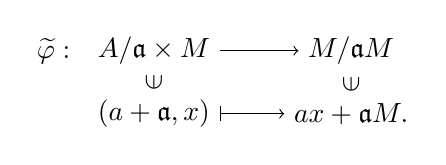
\begin{tikzpicture}[node distance=1mm]
  \node (functionName) at (0, 0) {$\widetilde{\varphi}:$};
  \node[right = of functionName] (domain)
    {$A/\mathfrak{a} \times M$};
  \node[below = 2mm of domain] (element) {$(a + \mathfrak{a}, x)$};
  \path (element)--(domain)node[midway,sloped] {$\in$};
  \node[right = 1cm of domain] (codomain) {$M/\mathfrak{a}M$};
  \node at (element-|codomain) (image) {$ax + \mathfrak{a}M.$};
  \path (image)--(codomain)node[midway,sloped] {$\in$};
  \draw[->] (domain) -- (codomain);
  \draw[|->] (element) -- (image);
\end{tikzpicture}
\end{center}
$\widetilde{\varphi}$ is well-defined and $A$-bilinear.
\item[(2)]
By the universal property,
$\widetilde{\varphi}$ factors through a $A$-bilinear map
$$\varphi: A/\mathfrak{a} \otimes_{A} M
\to M/\mathfrak{a}M$$
(such that $\varphi(a \otimes x) = \widetilde{\varphi}(a, x)$).
\item[(3)]
To show that $\varphi$ is isomorphic, might find the inverse map
$\psi: M/\mathfrak{a}M
\to
A/\mathfrak{a} \otimes_{A} M$
of $\varphi$.
Define $\psi$ by
\begin{center}
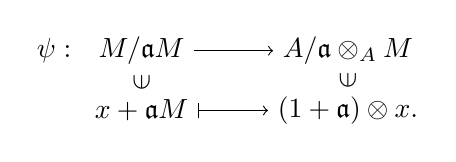
\begin{tikzpicture}[node distance=1mm]
  \node (functionName) at (0, 0) {$\psi:$};
  \node[right = of functionName] (domain) {$M/\mathfrak{a}M$};
  \node[below = 2mm of domain] (element) {$x + \mathfrak{a}M$};
  \path (element)--(domain)node[midway,sloped] {$\in$};
  \node[right = 1cm of domain] (codomain)
    {$A/\mathfrak{a} \otimes_{A} M$};
  \node at (element-|codomain) (image) {$(1 + \mathfrak{a}) \otimes x.$};
  \path (image)--(codomain)node[midway,sloped] {$\in$};
  \draw[->] (domain) -- (codomain);
  \draw[|->] (element) -- (image);
\end{tikzpicture}
\end{center}
$\psi$ is well-defined and $A$-linear.
\item[(4)]
$\psi \circ \varphi = \text{id}$.
\item[(5)]
$\varphi \circ \psi = \text{id}$.
\end{enumerate}
$\Box$ \\\\



%%%%%%%%%%%%%%%%%%%%%%%%%%%%%%%%%%%%%%%%%%%%%%%%%%%%%%%%%%%%%%%%%%%%%%%%%%%%%%%%



\textbf{Exercise 2.3.}
\emph{Let $A$ be a local ring, $M$ and $N$ finitely generated $A$-modules.
Prove that if $M \otimes_{A} N = 0$, then $M = 0$ or $N = 0$.
(Hint: Let $\mathfrak{m}$ be the maximal ideal,
$k = A/\mathfrak{m}$ the residue field.
Let $M_k = k \otimes_{A} M \cong M/\mathfrak{m}M$ by Exercise 2.2.
By Nakayama's lemma, $M_k = 0 \Longrightarrow M = 0$.
But
$M \otimes_{A} N = 0
\Longrightarrow
(M \otimes_{A} N)_k = 0
\Longrightarrow
M_k \otimes_k N_k = 0
\Longrightarrow
M_k = 0 \text{ or } N_k = 0$
since $M_k$, $N_k$ are vector spaces over a field.)} \\

The conclusion might be false if $A$ is not local. For example, Exercise 2.1. \\

\emph{Proof (Hint).}
Let $\mathfrak{m}$ be the maximal ideal,
$k = A/\mathfrak{m}$ the residue field.
Let $M_k = k \otimes_{A} M$.
\begin{enumerate}
\item[(1)]
\emph{(Base extension) Show that
$(M \otimes_{A} N)_k = M_k \otimes_{k} N_k$.}
In fact, by Proposition 2.14
\begin{align*}
(M \otimes_{A} N)_k
&= k \otimes_{A} (M \otimes_{A} N) \\
&= (k \otimes_{A} M) \otimes_{A} N \\
&= M_k \otimes_{A} N \\
&= (M_k \otimes_{k} k) \otimes_{A} N \\
&= M_k \otimes_{k} (k \otimes_{A} N) \\
&= M_k \otimes_{k} N_k.
\end{align*}
\item[(2)]
\begin{align*}
M \otimes_{A} N = 0
&\Longrightarrow
(M \otimes_{A} N)_k = 0 \\
&\Longrightarrow
M_k \otimes_k N_k = 0
  &\text{((1))} \\
&\Longrightarrow
M_k = 0 \text{ or } N_k = 0
  &\text{($M_k, N_k$: vector spaces)} \\
&\Longrightarrow
M/\mathfrak{m}M = 0 \text{ or } M/\mathfrak{m}M = 0
  &\text{(Exercise 2.2)} \\
&\Longrightarrow
M = 0 \text{ or } N = 0.
  &\text{(Nakayama's lemma)} \\
\end{align*}
\end{enumerate}
$\Box$ \\\\



%%%%%%%%%%%%%%%%%%%%%%%%%%%%%%%%%%%%%%%%%%%%%%%%%%%%%%%%%%%%%%%%%%%%%%%%%%%%%%%%



\textbf{Exercise 2.5.}
\emph{Let $A[x]$ be the ring of polynomials in one indeterminate over a ring $A$.
Prove that $A[x]$ is a flat $A$-algebra. (Hint: Use Exercise 2.4.)} \\

\emph{Proof (Hint).}
\begin{enumerate}
\item[(1)]
$A$ is a flat $A$-module by Proposition 2.14(iv).
\item[(2)]
As an $A$-module,
$$A[x]
\cong \bigoplus_{n \in \mathbb{Z}^+} Ax^n
\cong \bigoplus_{n \in \mathbb{Z}^+} A$$
(since $Ax^n \cong A$).
\item[(3)]
By Exercise 2.4, $A[x] \cong \bigoplus_{n \in \mathbb{Z}^+} A$ is flat.
\end{enumerate}
$\Box$ \\\\



%%%%%%%%%%%%%%%%%%%%%%%%%%%%%%%%%%%%%%%%%%%%%%%%%%%%%%%%%%%%%%%%%%%%%%%%%%%%%%%%



\textbf{Exercise 2.8.}
\begin{enumerate}
\item[(i)]
\emph{If $M$ and $N$ are flat $A$-modules, then so is $M \otimes_{A} N$. }
\item[(ii)]
\emph{If $B$ is a flat $A$-algebra and $N$ is a flat $B$-module,
then $N$ is flat as $A$-module.} \\
\end{enumerate}

\emph{Proof of (i).}
Given any exact sequence of $A$-modules
$0 \to N_1 \to N_2 \to N_3 \to 0$.
Since $M$ is flat,
$$0 \to N_1 \otimes_{A} M \to N_2 \otimes_{A} M \to N_3 \otimes_{A} M \to 0$$
is exact.
Since $N$ is flat,
$$0 \to (N_1 \otimes_{A} M) \otimes_{A} N
\to (N_2 \otimes_{A} M) \otimes_{A} N
\to (N_3 \otimes_{A} M) \otimes_{A} N \to 0$$
is exact.
By Proposition 2.14 (ii),
$$0 \to N_1 \otimes_{A} (M \otimes_{A} N)
\to N_2 \otimes_{A} (M \otimes_{A} N)
\to N_3 \otimes_{A} (M \otimes_{A} N) \to 0$$
is exact, or $M \otimes_{A} N$ is flat.
$\Box$ \\

\emph{Proof of (ii).}
Given any exact sequence of $A$-modules
$0 \to N_1 \to N_2 \to N_3 \to 0$.
Since $B$ is a flat $A$-algebra ($A$-module),
$$0 \to N_1 \otimes_{A} B \to N_2 \otimes_{A} B \to N_3 \otimes_{A} B \to 0$$
is exact.
Since $N$ is a flat $B$-module,
$$0 \to (N_1 \otimes_{A} B) \otimes_{B} N
\to (N_2 \otimes_{A} B) \otimes_{B} N
\to (N_3 \otimes_{A} B) \otimes_{B} N \to 0$$
is exact.
By ``Exercise 2.15'' on page 27,
$$0 \to N_1 \otimes_{A} (B \otimes_{B} N)
\to N_2 \otimes_{A} (B \otimes_{B} N)
\to N_3 \otimes_{A} (B \otimes_{B} N) \to 0$$
is exact.
By Proposition 2.14 (iv),
$$0 \to N_1 \otimes_{A} N
\to N_2 \otimes_{A} N
\to N_3 \otimes_{A} N \to 0$$
is exact,
or $N$ is flat.
$\Box$ \\\\



%%%%%%%%%%%%%%%%%%%%%%%%%%%%%%%%%%%%%%%%%%%%%%%%%%%%%%%%%%%%%%%%%%%%%%%%%%%%%%%%



\end{document}